\chapter{Results \& Discussions}
\indent\indent This chapter includes results obtained individually from object detection model, denoising autoencoder and text extraction, and the final result obtained after combining all models with text summarization. It also includes a text extraction and summarization comparison for pure and deblurred slide images.
\section{Object detection model}
This section includes training details, model accuracy and results obtained for object detection model.
\subsection{Training details}
% \ref{c6:tab1} Results of Object detection model
\begin{table}[H]
\centering
\fontsize{10}{12}\selectfont
\caption{Object detection Training}
\label{c6:tab1}
\small\addtolength{\tabcolsep}{40pt}
\def\arraystretch{1.5}
\begin{tabular}{|p{5cm}|p{2cm}|}
	\hline
% 	\multicolumn{2}{|c|}{Training} \\
	
% 	\hline
	\textbf{Number of epochs}   & 16000\\\hline
	\textbf{Training images used}&   320\\\hline
	\textbf{Validation images used} & 90\\\hline
	\textbf{Total loss}  &  0.035\\\hline
\end{tabular}
\end{table}
\subsection{Accuracy}
% \ref{fig:accuracy} 
\begin{figure}[H]
\centering
	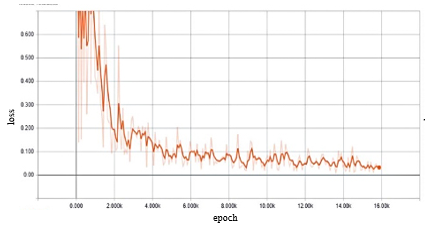
\includegraphics[scale=1]{Figures/ob_loss.png}	
	\caption{Object detection total loss}
	\label{fig:ob_loss}
\end{figure}

% \ref{fig:loss} 
\begin{figure}[H]
\centering
	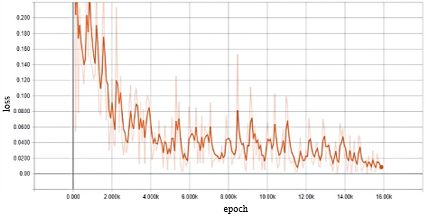
\includegraphics[scale=1]{Figures/ob_class.png}	
	\caption{Object detection classification loss}
	\label{fig:ob_class}
\end{figure}
\subsection{Result obtained}
% \ref{fig:detect1} 
\begin{figure}[H]
\centering
	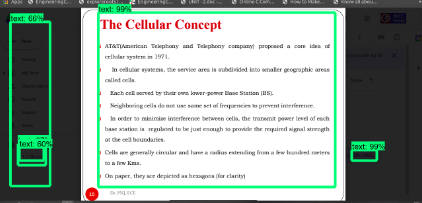
\includegraphics[scale=1]{Figures/detect1.png}	
	\caption{Object detection result}
	\label{fig:detect1}
\end{figure}

\section{Denoising Autoencoder}
This section includes training details, model accuracy and results obtained for denoising autoencoder.
\subsection{Training details}
\begin{table}[H]
\centering
\fontsize{10}{12}\selectfont
\caption{\acrlong{da} training}
\label{c6:tab2}
\small\addtolength{\tabcolsep}{40pt}
\def\arraystretch{1.5}
\begin{tabular}{|p{5cm}|p{2cm}|}
	\hline
% 	\multicolumn{2}{|c|}{Training} \\
	
% 	\hline
	\textbf{Number of epochs}   & 1000\\\hline
	\textbf{Training images used}&   280\\\hline
	\textbf{Validation images used} & 70\\\hline
	\textbf{Training accuracy}    &91\%\\\hline
	\textbf{Validation accuracy}&   87\%\\\hline
	\hline
\end{tabular}
\end{table}
\subsection{Training and validation accuracy}
% \ref{fig:accuracy} 
\begin{figure}[H]
\centering
	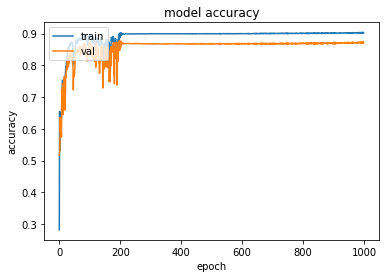
\includegraphics[scale=1]{Figures/denoise_accuracy.png}	
	\caption{\acrlong{da} Accuracy}
	\label{fig:denoise_accuracy}
\end{figure}
\subsection{Training and validation loss}
% \ref{fig:loss} 
\begin{figure}[H]
\centering
	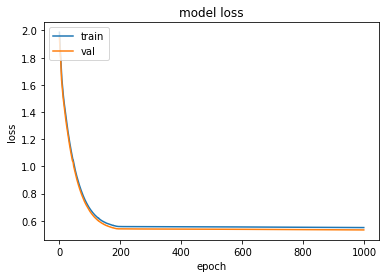
\includegraphics[scale=1]{Figures/denoise_loss.png}	
	\caption{\acrlong{da} Loss}
	\label{fig:denoise_loss}
\end{figure}
\subsection{Result obtained}
% \ref{fig:denoise} 
\begin{figure}[H]
\centering
	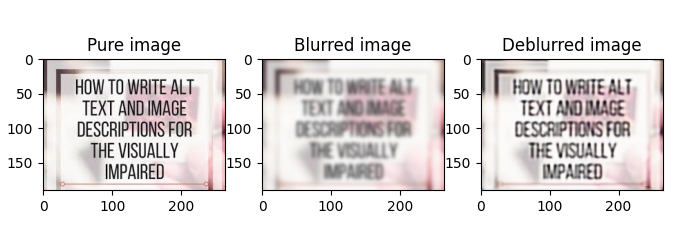
\includegraphics[scale=0.7]{Figures/denoise1.png}	
	\caption{\acrlong{da} output}
	\label{fig:denoise}
\end{figure}

\section{Text Extraction}
This section includes results obtained from text extraction method for a pure, blurred and deblurred image.
\subsection{Text extraction for pure image}
% \ref{fig:pure} 
\begin{figure}[H]
\centering
	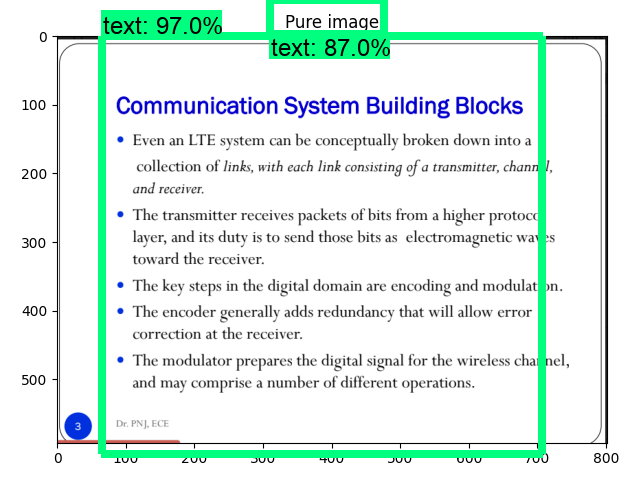
\includegraphics[scale=0.7]{Figures/myplot_pure.png}	
	\caption{Pure image}
	\label{fig:pure}
\end{figure}
% \ref{fig:pure_op} 
\begin{figure}[H]
\centering
	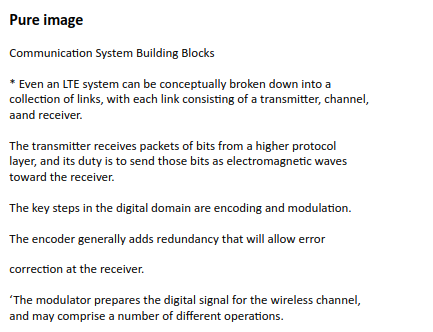
\includegraphics[scale=0.7]{Figures/pure_op.png}	
	\caption{Text Extracted from pure image}
	\label{fig:pure_op}
\end{figure}

\subsection{Text extraction for blurred image}
% \ref{fig:blur} 
\begin{figure}[H]
\centering
	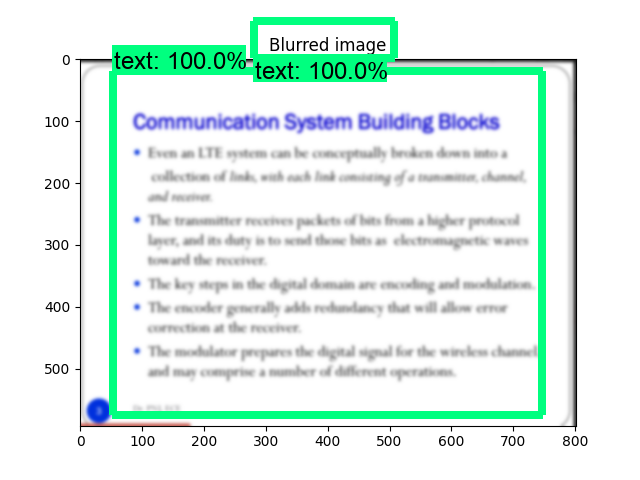
\includegraphics[scale=0.7]{Figures/myplot_blur.png}	
	\caption{Blurred image}
	\label{fig:blur}
\end{figure}
% \ref{fig:blur_op} 
\begin{figure}[H]
\centering
	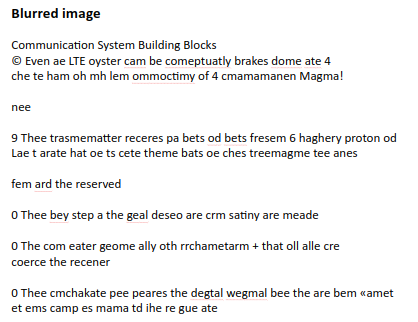
\includegraphics[scale=0.7]{Figures/blur_op.png}	
	\caption{Text Extracted from blurred image}
	\label{fig:blur_op}
\end{figure}

\subsection{Text extraction for deblurred image}
% \ref{fig:deblur} 
\begin{figure}[H]
\centering
	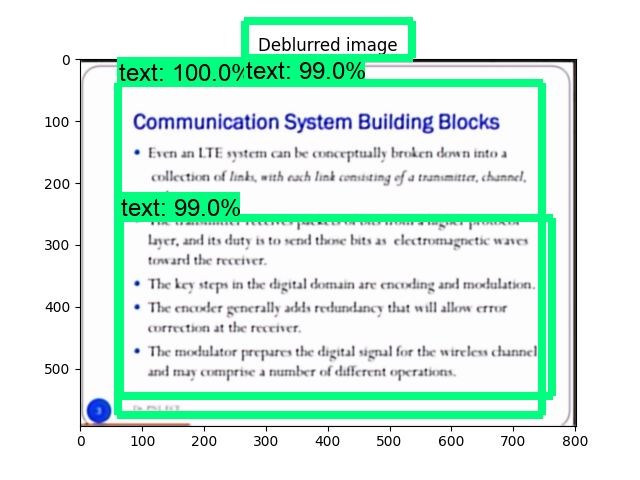
\includegraphics[scale=0.7]{Figures/myplot_deblur.png}	
	\caption{Deblurred image}
	\label{fig:deblur}
\end{figure}
% \ref{fig:deblur_op} 
\begin{figure}[H]
\centering
	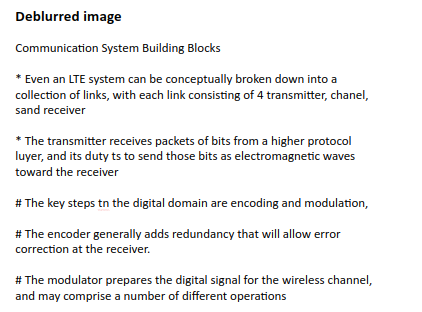
\includegraphics[scale=0.7]{Figures/deblur_op.png}	
	\caption{Text Extracted from deblurred image}
	\label{fig:deblur_op}
\end{figure}
\newpage
\section{Summarization}

\subsection{Summarization of text extracted from pure slides}
Extracted text from pure slides is shown in figure \ref{fig:orig_text2}.
\begin{figure}[H]
\centering
	\makebox[\textwidth]{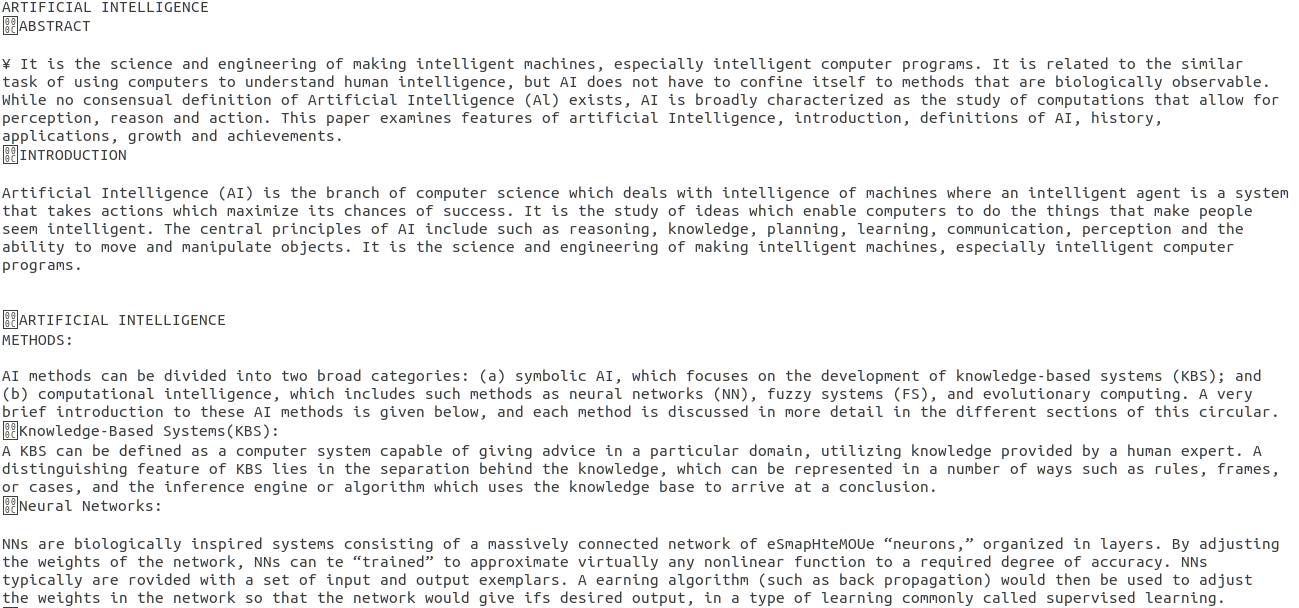
\includegraphics[scale=0.45]{Figures/orig_text1.png}}
% 	\caption{Text extracted from pure slides}
	\label{fig:orig_text1}
\end{figure}
% \ref{fig:deblur_op} 
\begin{figure}[H]
\centering
	\makebox[\textwidth]{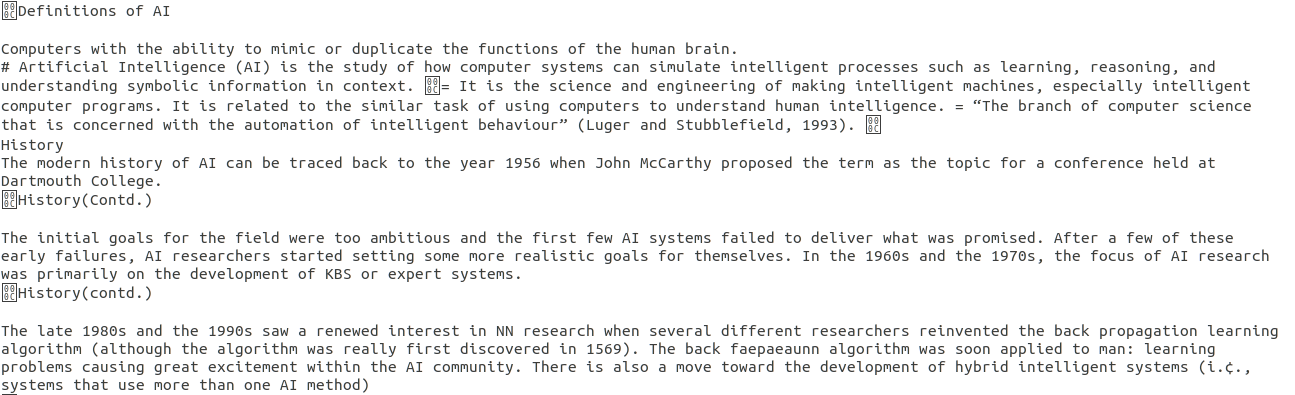
\includegraphics[scale=0.45]{Figures/orig_text2.png}}	
	\caption{Text extracted from pure slides}
	\label{fig:orig_text2}
\end{figure}
\newpage
Summary generated for the above text is shown in figure \ref{fig:orig_sum1}.
\begin{figure}[H]
\centering
	\makebox[\textwidth]{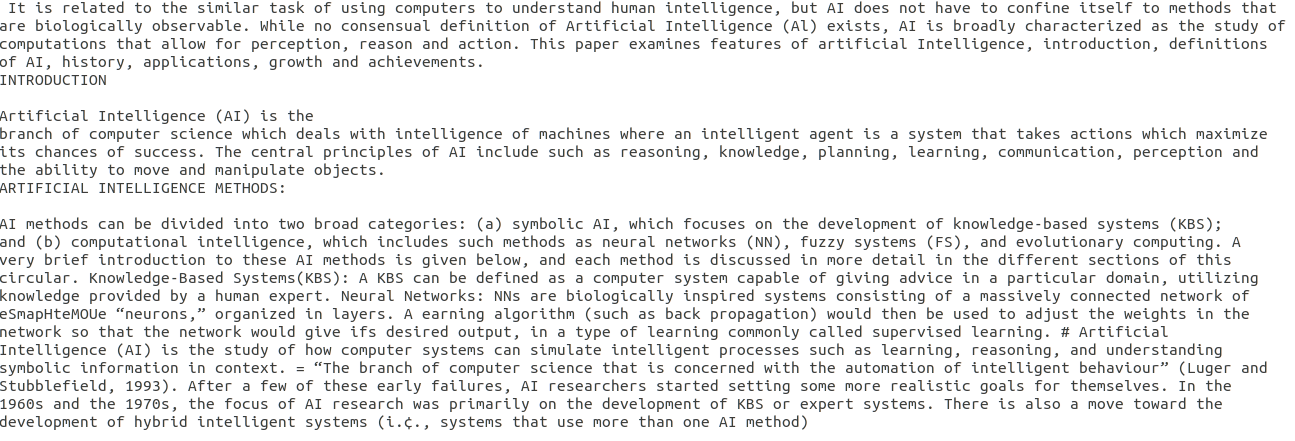
\includegraphics[scale=0.45]{Figures/orig_sum1.png}}	
	\caption{Text summarized from pure slides}
	\label{fig:orig_sum1}
\end{figure}

\subsection{Summarization of text extracted from deblurred slides}
Extracted text from deblurred slides is shown in figure \ref{fig:deblur_text2}.
\begin{figure}[H]
\centering
	\makebox[\textwidth]{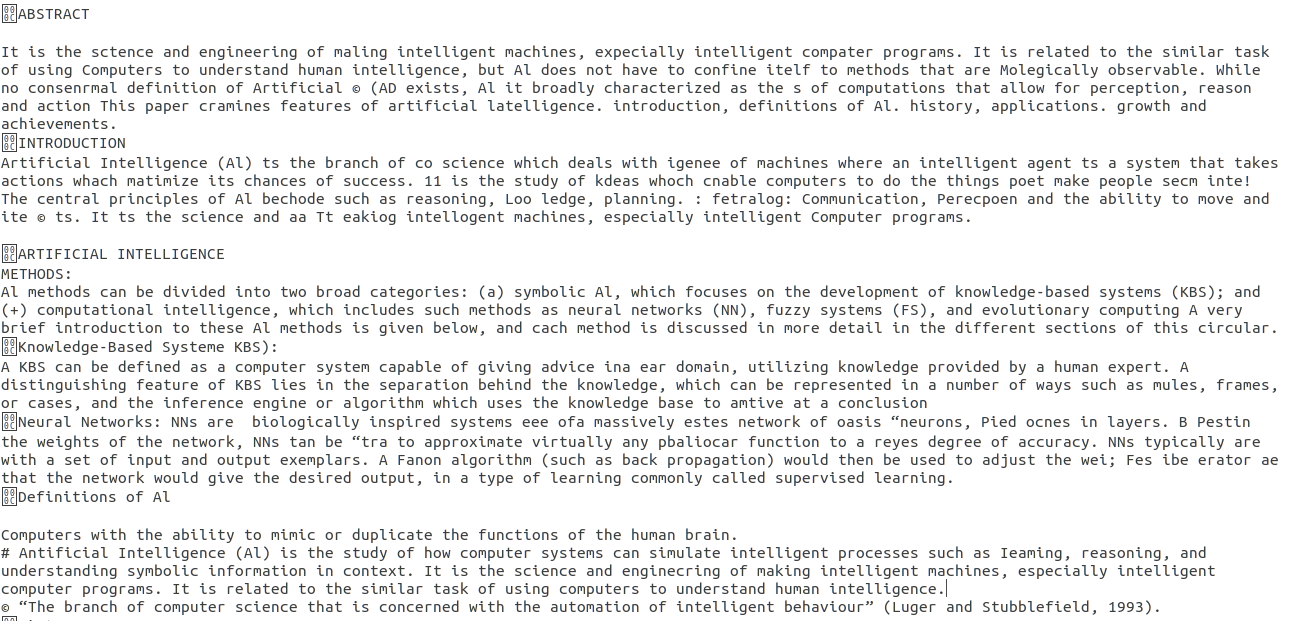
\includegraphics[scale=0.45]{Figures/deblur_text1.png}}
% 	\caption{Text extracted from pure slides}
	\label{fig:deblur_text1}
\end{figure}
% \ref{fig:deblur_op} 
\begin{figure}[H]
\centering
	\makebox[\textwidth]{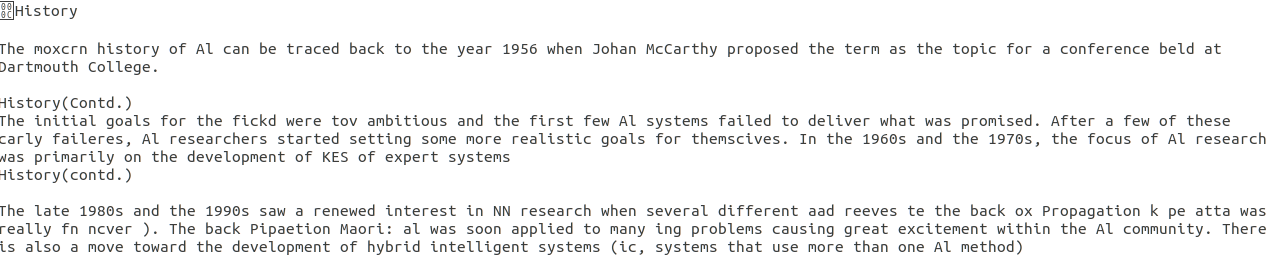
\includegraphics[scale=0.45]{Figures/deblur_text2.png}}	
	\caption{Text extracted from deblurred slides}
	\label{fig:deblur_text2}
\end{figure}
% \newpage
Summary generated for the above text is shown in figure \ref{fig:deblur_sum1}.
\begin{figure}[H]
\centering
	\makebox[\textwidth]{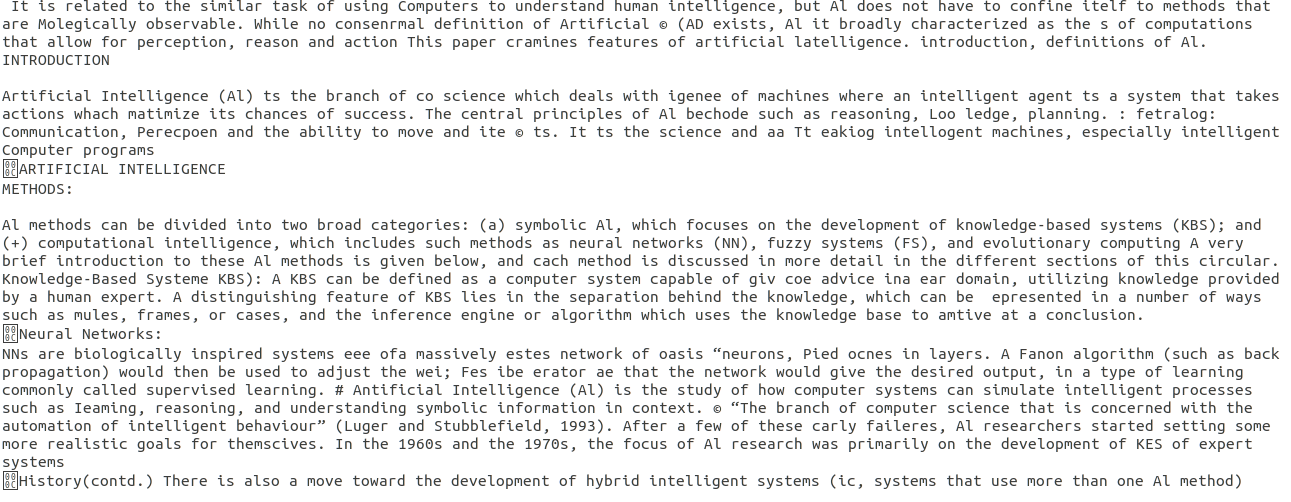
\includegraphics[scale=0.45]{Figures/deblur_sum1.png}}	
	\caption{Text summarized from deblurred slides}
	\label{fig:deblur_sum1}
\end{figure}

To summarize, this chapter gives independent results obtained for each trained model. Final section gives the result obtained after combining all the models. It also gives a comparison of results obtained for pure, blurred and deblurred images where deblurring is achieved using denoising autoencoder.




